\documentclass{article}
\usepackage[backend=biber,natbib=true,style=alphabetic,maxbibnames=50]{biblatex}
\addbibresource{/home/nqbh/reference/bib.bib}
\usepackage[utf8]{vietnam}
\usepackage{tocloft}
\renewcommand{\cftsecleader}{\cftdotfill{\cftdotsep}}
\usepackage[colorlinks=true,linkcolor=blue,urlcolor=red,citecolor=magenta]{hyperref}
\usepackage{amsmath,amssymb,amsthm,float,graphicx,mathtools,tikz}
\usetikzlibrary{angles,calc,intersections,matrix,patterns,quotes,shadings}
\allowdisplaybreaks
\newtheorem{assumption}{Assumption}
\newtheorem{baitoan}{}
\newtheorem{cauhoi}{Câu hỏi}
\newtheorem{conjecture}{Conjecture}
\newtheorem{corollary}{Corollary}
\newtheorem{dangtoan}{Dạng toán}
\newtheorem{definition}{Definition}
\newtheorem{dinhly}{Định lý}
\newtheorem{dinhnghia}{Định nghĩa}
\newtheorem{example}{Example}
\newtheorem{ghichu}{Ghi chú}
\newtheorem{hequa}{Hệ quả}
\newtheorem{hypothesis}{Hypothesis}
\newtheorem{lemma}{Lemma}
\newtheorem{luuy}{Lưu ý}
\newtheorem{nhanxet}{Nhận xét}
\newtheorem{notation}{Notation}
\newtheorem{note}{Note}
\newtheorem{principle}{Principle}
\newtheorem{problem}{Problem}
\newtheorem{proposition}{Proposition}
\newtheorem{question}{Question}
\newtheorem{remark}{Remark}
\newtheorem{theorem}{Theorem}
\newtheorem{vidu}{Ví dụ}
\usepackage[left=1cm,right=1cm,top=5mm,bottom=5mm,footskip=4mm]{geometry}
\def\labelitemii{$\circ$}
\DeclareRobustCommand{\divby}{%
	\mathrel{\vbox{\baselineskip.65ex\lineskiplimit0pt\hbox{.}\hbox{.}\hbox{.}}}%
}

\title{Problem: Visual Geometry -- Bài Tập: Hình Học Trực Quan}
\author{Nguyễn Quản Bá Hồng\footnote{Independent Researcher, Ben Tre City, Vietnam\\e-mail: \texttt{nguyenquanbahong@gmail.com}; website: \url{https://nqbh.github.io}.}}
\date{\today}

\begin{document}
\maketitle
\begin{abstract}
	Last updated version: \href{https://github.com/NQBH/elementary_STEM_beyond/blob/main/elementary_mathematics/grade_6/visual_geometry/problem/NQBH_visual_geometry_problem.pdf}{GitHub{\tt/}NQBH{\tt/}elementary STEM \& beyond{\tt/}elementary mathematics{\tt/}grade 6{\tt/}visual geometry{\tt/}problem: set $\mathbb{Q}$ of visual geometrys [pdf]}.\footnote{\textsc{url}: \url{https://github.com/NQBH/elementary_STEM_beyond/blob/main/elementary_mathematics/grade_6/visual_geometry/problem/NQBH_visual_geometry_problem.pdf}.} [\href{https://github.com/NQBH/elementary_STEM_beyond/blob/main/elementary_mathematics/grade_6/visual_geometry/problem/NQBH_visual_geometry_problem.tex}{\TeX}]\footnote{\textsc{url}: \url{https://github.com/NQBH/elementary_STEM_beyond/blob/main/elementary_mathematics/grade_6/rational/problem/NQBH_visual_geometry_problem.tex}.}. 
\end{abstract}
\tableofcontents

%------------------------------------------------------------------------------%

\section{Rectangle. Square -- Hình Chữ Nhật. Hình Vuông}

\begin{baitoan}[\cite{Tuyen_Toan_6}, Ví dụ 1, p. 75]
	Trong hình sau có bao nhiêu: (a) Hình vuông? (b) Hình chữ nhật?
	\begin{center}
		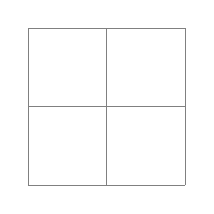
\begin{tikzpicture}
			\centering
			\draw[step=1,gray,very thin](0,0) grid (2,2);
		\end{tikzpicture}
	\end{center}	
\end{baitoan}

\begin{baitoan}[\cite{Tuyen_Toan_6}, 1., p. 76]
	Vẽ đoạn thẳng $AB = 4$ {\rm cm} rồi vẽ hình vuông AMBN nhận AB làm 1 đường chéo.
\end{baitoan}

\begin{baitoan}[\cite{Tuyen_Toan_6}, 2., p. 76]
	Vẽ 1 hình vuông lên giấy sau đó cắt hình vuông này thành 4 phần bằng nhau rồi ghép lại thành 2 hình vuông.
\end{baitoan}

\begin{baitoan}[\cite{Tuyen_Toan_6}, 3., p. 76]
	Vẽ đoạn thẳng $AB = 2$ {\rm cm}. (a) Vẽ 2 hình vuông ABCD \& ABEF chung cạnh AB. (b) Tứ giác FDCE là hình gì? Tính các cạnh của FDCE.
\end{baitoan}

\begin{baitoan}[\cite{Tuyen_Toan_6}, 4., p. 76]
	Từ các hình vuông nhỏ cạnh {\rm1 cm}, xếp chúng liền kề nhau thành 1 hình chữ nhật có các cạnh $\ge2$ {\rm cm}. Gọi $n$ là số các hình vuông nhỏ được dùng. Hỏi $n$ là các số nào?
\end{baitoan}

\begin{baitoan}[\cite{Tuyen_Toan_6}, 5., p. 76]
	Vẽ hình theo sự diễn đạt: (a) Vẽ hình chữ nhật ABCD sao cho $CD = 6$ {\rm cm}, $AD = 2$ {\rm cm}. (b) Vẽ hình vuông AMND vào trong hình chữ nhật ABCD. So sánh MN \& BC.
\end{baitoan}

%------------------------------------------------------------------------------%

\section{Parallelogram. Rhombus -- Hình Bình Hành. Hình Thoi}

\begin{baitoan}[\cite{Tuyen_Toan_6}, Ví dụ 2., p. 77]
	Có 1 hình bình hành ABCD bằng bìa, cạnh $AB = 5$ {\rm cm}, cạnh $BC = 2$ {\rm cm}. Dùng kéo cắt 1 nhát để được 1 hình bình hành \& 1 hình thoi. Xác định vị trí của nhát cắt.
\end{baitoan}

\begin{baitoan}[\cite{Tuyen_Toan_6}, 6., p. 77]
	Có 2 loại êke: loại êke $60^\circ$ \& loại êke $45^\circ$. Dùng 2 êke bằng nhau để ghép thành: (a) 1 hình chữ nhật. (b) 1 hình bình hành. (c) 1 hình thoi.
\end{baitoan}

\begin{baitoan}[\cite{Tuyen_Toan_6}, 7., p. 77]
	Vẽ hình bình hành ABCD sao cho $AB = 2$ {\rm cm}, $BC = 3$ {\rm cm}, \& $CA = 4$ {\rm cm}.
\end{baitoan}

\begin{baitoan}[\cite{Tuyen_Toan_6}, 8., p. 77]
	Vẽ hình thoi ABCD sao cho $AC = 6$ {\rm cm} \& $BD = 3$ {\rm cm}.
\end{baitoan}

\begin{baitoan}[\cite{Tuyen_Toan_6}, 9., p. 77]
	Vẽ hình thoi ABCD sao cho độ dài mỗi cạnh là {\rm3 cm} có $\widehat{A} = 50^\circ$.
\end{baitoan}

\begin{baitoan}[\cite{Tuyen_Toan_6}, 10., p. 77]
	Cho 7 điểm $A,B,C,D,E,F,G$. Viết các nhóm 4 điểm trong 7 điểm đó là 4 đỉnh của: (a) 1 hình chữ nhật. (b) 1 hình bình hành nhưng không là hình chữ nhật.
	\begin{center}
		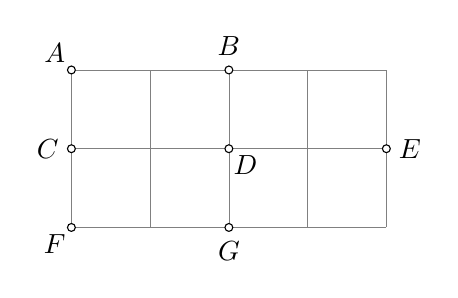
\begin{tikzpicture}
			\centering
			\draw[step=1,gray,very thin](0,0) grid (4,2);
			\path
			(0,2) coordinate (A)
			(2,2) coordinate (B)
			(0,1) coordinate (C)
			(2,1) coordinate (D)
			(4,1) coordinate (E)
			(0,0) coordinate (F)
			(2,0) coordinate (G)
			;
			\foreach \x/\g in {A/135,B/90,C/180,D/-45,E/0,F/-135,G/-90} \draw[fill=white] (\x) circle (.05) + (\g:.3) node{$\x$};
		\end{tikzpicture}
	\end{center}
\end{baitoan}


%------------------------------------------------------------------------------%

\section{Miscellaneous}

%------------------------------------------------------------------------------%

\printbibliography[heading=bibintoc]

\end{document}